\documentclass{article}
\usepackage[utf8]{inputenc}
\usepackage{amsmath}
\usepackage{graphicx}


\begin{document}

\begin{titlepage}
\centering
{\LARGE\bfseries Lab 01: Hybrid Encryption}

\vspace{1cm}

{\large 21120263 - Tong Nguyen Minh Khang}

\vfill

{\itshape University of Science - HCMUS}

\vspace{0.5cm}
{CSC15106 – Knowledge Engineering Seminar}

\end{titlepage}

\section{Introduction}
This report describes a simple hybrid encryption system for secure file exchange.

\section{Architecture}

\begin{figure}[h]
    \centering
    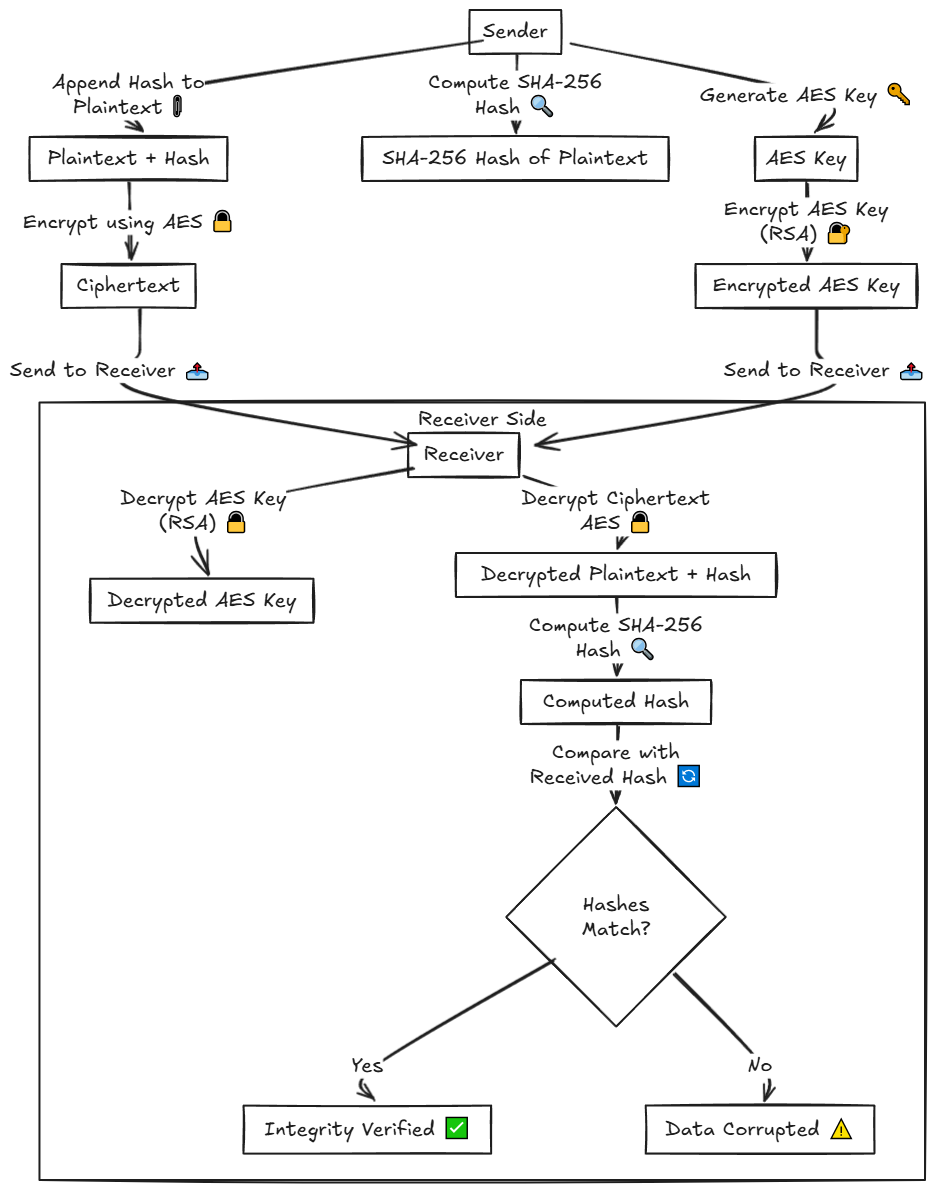
\includegraphics[width=0.95\textwidth]{diagram.png}
    \caption{Flow during encryption and decryption.}
    \label{fig:sample}
\end{figure}

\subsection*{Sender Side}

\begin{enumerate}
    \item \textbf{Compute SHA-256 Hash}: 
    The sender computes the SHA-256 hash of the plaintext message.

    \item \textbf{Append Hash to Plaintext}:
    The computed hash is appended to the plaintext, forming a combined message: \textit{Plaintext + Hash}.

    \item \textbf{Generate AES Key}:
    An AES key is generated for encrypting the plaintext.

    \item \textbf{Encrypt Plaintext and Hash}:
    The combined \textit{Plaintext + Hash} is encrypted using the AES key, resulting in the ciphertext.

    \item \textbf{Encrypt AES Key}:
    The AES key is encrypted using RSA encryption to ensure secure key exchange.

    \item \textbf{Send to Receiver}:
    The sender transmits the encrypted AES key and the ciphertext to the receiver.
\end{enumerate}

\subsection*{Receiver Side}

\begin{enumerate}
    \item \textbf{Receive Data}:
    The receiver obtains the encrypted AES key and the ciphertext.

    \item \textbf{Decrypt AES Key}:
    The receiver uses RSA decryption to recover the AES key.

    \item \textbf{Decrypt Ciphertext}:
    The ciphertext is decrypted using the recovered AES key, resulting in the original \textit{Plaintext + Hash}.

    \item \textbf{Compute SHA-256 Hash}:
    The receiver extracts the plaintext and computes its SHA-256 hash.

    \item \textbf{Compare Hashes}:
    The receiver compares the computed hash with the hash received along with the plaintext.

    \item \textbf{Verify Integrity}:
    If the computed hash matches the received hash, data integrity is verified, and the process concludes successfully.
    If the hashes do not match, the data is identified as corrupted.
\end{enumerate}

\subsection*{Final Result}

- If the hashes match, the process confirms that the data has not been tampered with, and the integrity is verified. \\
- If the hashes do not match, it indicates data corruption during transmission. \\

\section{System Overview}
The system consists of the following main components:

\begin{itemize}
    \item \textbf{RSA Encryption:} Used to encrypt the symmetric AES key.
    \item \textbf{AES Encryption:} Used for the encryption of the actual file data.
    \item \textbf{Hashing using SHA-256:} Applied to ensure data integrity by checking the hash of the encrypted file against that of the decrypted file. 
\end{itemize}

\section{Special Parameters}
The following parameters are used in the program:
\begin{itemize}
    \item \textbf{RSA Key Size:} A standard of 2048 bits is used for generating RSA key pairs.
    \item \textbf{AES Key Size:} An AES block size of 16 bytes (128 bits) is utilized for encrypting the data.
    \item \textbf{Hash Algorithm:} The SHA-256 hash function is employed to verify the integrity of the encrypted data.
    \item \textbf{Supported File Types:} The system is designed to handle various binary files for encryption and decryption, with no explicit limitations on file types within the binary format, as long as you have permissions to read the input file (key and unencrypted file), and writing the output files (encrypted file, decrypted file, encrypted key, public and private keys) to the directory you specified.
\end{itemize}

\section{References}


\end{document}